% SOURCE: ../../edit-harness/results/merging/RG_gain_law_20260715.json
% !TEX encoding = UTF-8 Unicode
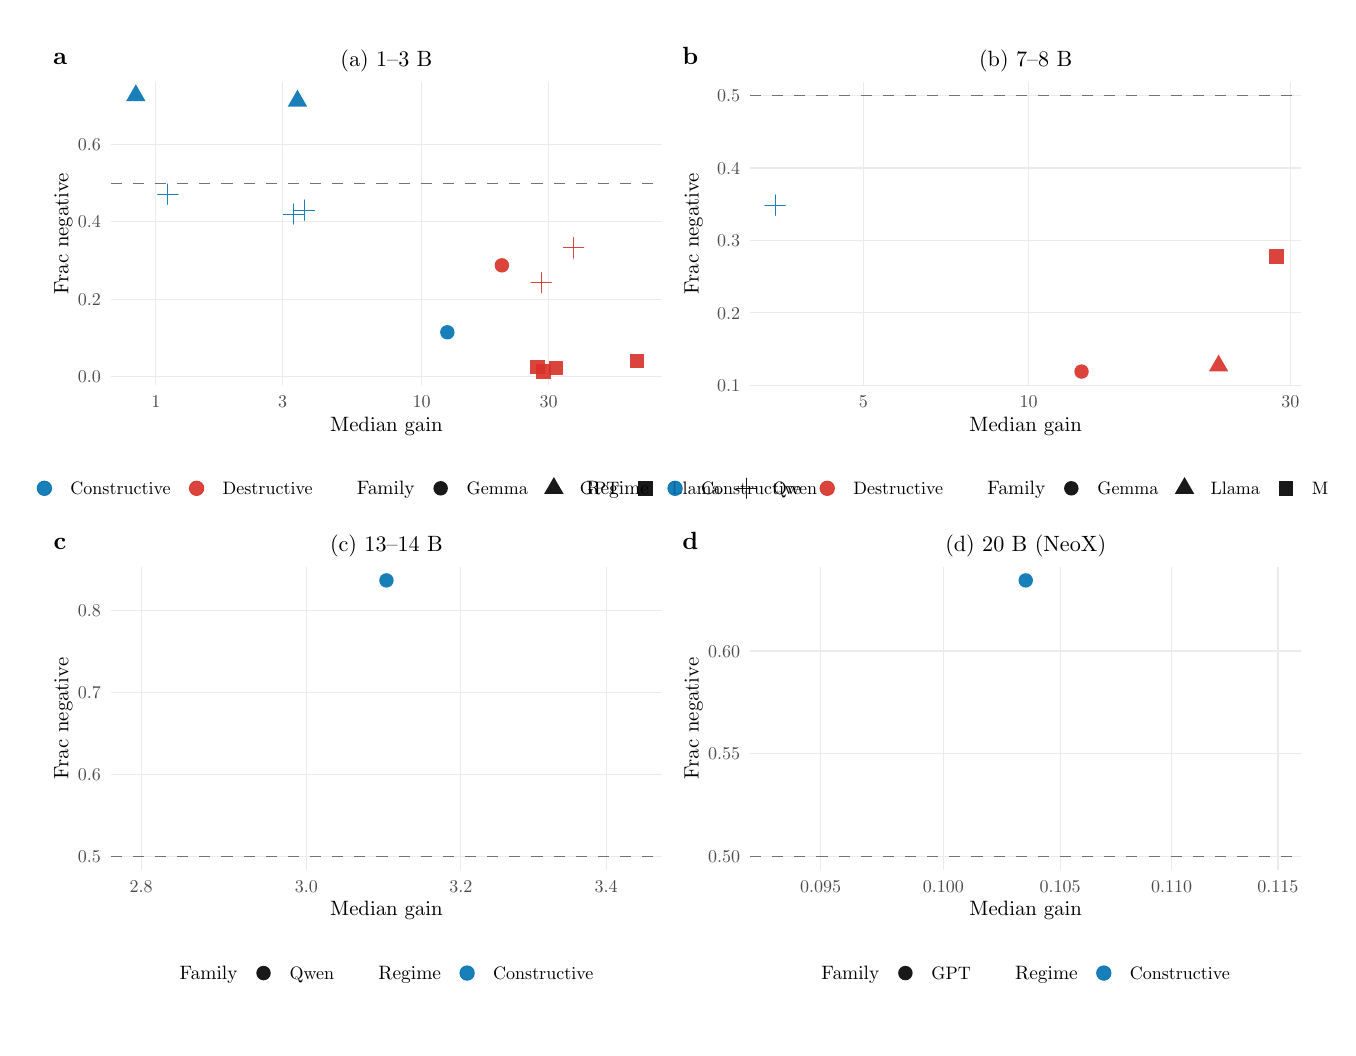
\begin{tikzpicture}[x=1pt,y=1pt]
\definecolor{fillColor}{RGB}{255,255,255}
\path[use as bounding box,fill=fillColor,fill opacity=0.00] (0,0) rectangle (469.75,361.35);
\begin{scope}
\path[clip] (  0.00,  0.00) rectangle (469.75,361.35);
\definecolor{drawColor}{RGB}{255,255,255}
\definecolor{fillColor}{RGB}{255,255,255}

\path[draw=drawColor,line width= 0.6pt,line join=round,line cap=round,fill=fillColor] (  0.00,  0.00) rectangle (469.76,361.35);
\end{scope}
\begin{scope}
\path[clip] (  5.50,180.68) rectangle (233.25,355.85);
\definecolor{fillColor}{RGB}{255,255,255}

\path[fill=fillColor] (  5.50,180.68) rectangle (233.25,355.85);
\end{scope}
\begin{scope}
\path[clip] (233.25,180.68) rectangle (464.25,355.85);
\definecolor{fillColor}{RGB}{255,255,255}

\path[fill=fillColor] (233.25,180.68) rectangle (464.25,355.85);
\end{scope}
\begin{scope}
\path[clip] (  5.50,  5.50) rectangle (233.25,180.68);
\definecolor{fillColor}{RGB}{255,255,255}

\path[fill=fillColor] (  5.50,  5.50) rectangle (233.25,180.68);
\end{scope}
\begin{scope}
\path[clip] (233.25,  5.50) rectangle (464.25,180.68);
\definecolor{fillColor}{RGB}{255,255,255}

\path[fill=fillColor] (233.25,  5.50) rectangle (464.25,180.68);
\end{scope}
\begin{scope}
\path[clip] ( 30.03,232.09) rectangle (229.25,341.79);
\definecolor{drawColor}{gray}{0.92}

\path[draw=drawColor,line width= 0.4pt,line join=round] ( 30.03,235.22) --
	(229.25,235.22);

\path[draw=drawColor,line width= 0.4pt,line join=round] ( 30.03,263.23) --
	(229.25,263.23);

\path[draw=drawColor,line width= 0.4pt,line join=round] ( 30.03,291.24) --
	(229.25,291.24);

\path[draw=drawColor,line width= 0.4pt,line join=round] ( 30.03,319.25) --
	(229.25,319.25);

\path[draw=drawColor,line width= 0.4pt,line join=round] ( 46.29,232.09) --
	( 46.29,341.79);

\path[draw=drawColor,line width= 0.4pt,line join=round] ( 92.14,232.09) --
	( 92.14,341.79);

\path[draw=drawColor,line width= 0.4pt,line join=round] (142.39,232.09) --
	(142.39,341.79);

\path[draw=drawColor,line width= 0.4pt,line join=round] (188.24,232.09) --
	(188.24,341.79);
\definecolor{fillColor}{RGB}{215,48,39}

\path[fill=fillColor,fill opacity=0.90] (181.54,236.10) --
	(186.77,236.10) --
	(186.77,241.33) --
	(181.54,241.33) --
	cycle;

\path[fill=fillColor,fill opacity=0.90] (183.72,234.46) --
	(188.95,234.46) --
	(188.95,239.69) --
	(183.72,239.69) --
	cycle;

\path[fill=fillColor,fill opacity=0.90] (217.58,238.30) --
	(222.81,238.30) --
	(222.81,243.53) --
	(217.58,243.53) --
	cycle;

\path[fill=fillColor,fill opacity=0.90] (188.33,235.70) --
	(193.56,235.70) --
	(193.56,240.93) --
	(188.33,240.93) --
	cycle;
\definecolor{drawColor}{RGB}{215,48,39}

\path[draw=drawColor,draw opacity=0.90,line width= 0.3pt,line join=round,line cap=round] (181.88,269.17) -- (189.28,269.17);

\path[draw=drawColor,draw opacity=0.90,line width= 0.3pt,line join=round,line cap=round] (185.58,265.47) -- (185.58,272.86);
\definecolor{drawColor}{RGB}{0,114,178}

\path[draw=drawColor,draw opacity=0.90,line width= 0.3pt,line join=round,line cap=round] ( 92.41,294.00) -- ( 99.80,294.00);

\path[draw=drawColor,draw opacity=0.90,line width= 0.3pt,line join=round,line cap=round] ( 96.11,290.30) -- ( 96.11,297.70);

\path[draw=drawColor,draw opacity=0.90,line width= 0.3pt,line join=round,line cap=round] ( 46.96,301.18) -- ( 54.35,301.18);

\path[draw=drawColor,draw opacity=0.90,line width= 0.3pt,line join=round,line cap=round] ( 50.65,297.48) -- ( 50.65,304.88);
\definecolor{drawColor}{RGB}{215,48,39}

\path[draw=drawColor,draw opacity=0.90,line width= 0.3pt,line join=round,line cap=round] (193.56,281.77) -- (200.96,281.77);

\path[draw=drawColor,draw opacity=0.90,line width= 0.3pt,line join=round,line cap=round] (197.26,278.07) -- (197.26,285.47);
\definecolor{drawColor}{RGB}{0,114,178}

\path[draw=drawColor,draw opacity=0.90,line width= 0.3pt,line join=round,line cap=round] ( 96.34,295.41) -- (103.74,295.41);

\path[draw=drawColor,draw opacity=0.90,line width= 0.3pt,line join=round,line cap=round] (100.04,291.71) -- (100.04,299.11);

\path[fill=fillColor,fill opacity=0.90] (171.35,275.47) circle (  2.61);
\definecolor{fillColor}{RGB}{0,114,178}

\path[fill=fillColor,fill opacity=0.90] (151.64,251.28) circle (  2.61);

\path[fill=fillColor,fill opacity=0.90] ( 97.49,338.92) --
	(101.01,332.82) --
	( 93.97,332.82) --
	cycle;

\path[fill=fillColor,fill opacity=0.90] ( 39.08,340.87) --
	( 42.60,334.77) --
	( 35.56,334.77) --
	cycle;
\definecolor{drawColor}{gray}{0.45}

\path[draw=drawColor,line width= 0.3pt,dash pattern=on 4pt off 4pt ,line join=round] ( 30.03,305.24) -- (229.25,305.24);
\end{scope}
\begin{scope}
\path[clip] (  0.00,  0.00) rectangle (469.75,361.35);
\definecolor{drawColor}{gray}{0.30}

\node[text=drawColor,anchor=base east,inner sep=0pt, outer sep=0pt, scale=  0.65] at ( 26.43,232.98) {0.0};

\node[text=drawColor,anchor=base east,inner sep=0pt, outer sep=0pt, scale=  0.65] at ( 26.43,260.99) {0.2};

\node[text=drawColor,anchor=base east,inner sep=0pt, outer sep=0pt, scale=  0.65] at ( 26.43,289.00) {0.4};

\node[text=drawColor,anchor=base east,inner sep=0pt, outer sep=0pt, scale=  0.65] at ( 26.43,317.01) {0.6};
\end{scope}
\begin{scope}
\path[clip] (  0.00,  0.00) rectangle (469.75,361.35);
\definecolor{drawColor}{gray}{0.30}

\node[text=drawColor,anchor=base,inner sep=0pt, outer sep=0pt, scale=  0.65] at ( 46.29,224.02) {1};

\node[text=drawColor,anchor=base,inner sep=0pt, outer sep=0pt, scale=  0.65] at ( 92.14,224.02) {3};

\node[text=drawColor,anchor=base,inner sep=0pt, outer sep=0pt, scale=  0.65] at (142.39,224.02) {10};

\node[text=drawColor,anchor=base,inner sep=0pt, outer sep=0pt, scale=  0.65] at (188.24,224.02) {30};
\end{scope}
\begin{scope}
\path[clip] (  0.00,  0.00) rectangle (469.75,361.35);
\definecolor{drawColor}{RGB}{0,0,0}

\node[text=drawColor,anchor=base,inner sep=0pt, outer sep=0pt, scale=  0.75] at (129.64,215.59) {Median gain};
\end{scope}
\begin{scope}
\path[clip] (  0.00,  0.00) rectangle (469.75,361.35);
\definecolor{drawColor}{RGB}{0,0,0}

\node[text=drawColor,rotate= 90.00,anchor=base,inner sep=0pt, outer sep=0pt, scale=  0.75] at ( 14.67,286.94) {Frac negative};
\end{scope}
\begin{scope}
\path[clip] (  0.00,  0.00) rectangle (469.75,361.35);
\definecolor{drawColor}{RGB}{0,0,0}

\node[text=drawColor,anchor=base west,inner sep=0pt, outer sep=0pt, scale=  0.70] at (-26.02,192.49) {Regime};
\end{scope}
\begin{scope}
\path[clip] (  0.00,  0.00) rectangle (469.75,361.35);
\definecolor{drawColor}{RGB}{0,114,178}
\definecolor{fillColor}{RGB}{0,114,178}

\path[draw=drawColor,draw opacity=0.90,line width= 0.3pt,line join=round,line cap=round,fill=fillColor,fill opacity=0.90] (  6.04,194.90) circle (  2.61);
\end{scope}
\begin{scope}
\path[clip] (  0.00,  0.00) rectangle (469.75,361.35);
\definecolor{drawColor}{RGB}{215,48,39}
\definecolor{fillColor}{RGB}{215,48,39}

\path[draw=drawColor,draw opacity=0.90,line width= 0.3pt,line join=round,line cap=round,fill=fillColor,fill opacity=0.90] ( 61.04,194.90) circle (  2.61);
\end{scope}
\begin{scope}
\path[clip] (  0.00,  0.00) rectangle (469.75,361.35);
\definecolor{drawColor}{RGB}{0,0,0}

\node[text=drawColor,anchor=base west,inner sep=0pt, outer sep=0pt, scale=  0.65] at ( 15.46,192.66) {Constructive};
\end{scope}
\begin{scope}
\path[clip] (  0.00,  0.00) rectangle (469.75,361.35);
\definecolor{drawColor}{RGB}{0,0,0}

\node[text=drawColor,anchor=base west,inner sep=0pt, outer sep=0pt, scale=  0.65] at ( 70.46,192.66) {Destructive};
\end{scope}
\begin{scope}
\path[clip] (  0.00,  0.00) rectangle (469.75,361.35);
\definecolor{drawColor}{RGB}{0,0,0}

\node[text=drawColor,anchor=base west,inner sep=0pt, outer sep=0pt, scale=  0.70] at (118.92,192.49) {Family};
\end{scope}
\begin{scope}
\path[clip] (  0.00,  0.00) rectangle (469.75,361.35);
\definecolor{fillColor}{RGB}{0,0,0}

\path[fill=fillColor,fill opacity=0.90] (149.23,194.90) circle (  2.61);
\end{scope}
\begin{scope}
\path[clip] (  0.00,  0.00) rectangle (469.75,361.35);
\definecolor{fillColor}{RGB}{0,0,0}

\path[fill=fillColor,fill opacity=0.90] (190.14,198.97) --
	(193.66,192.87) --
	(186.62,192.87) --
	cycle;
\end{scope}
\begin{scope}
\path[clip] (  0.00,  0.00) rectangle (469.75,361.35);
\definecolor{fillColor}{RGB}{0,0,0}

\path[fill=fillColor,fill opacity=0.90] (220.58,192.29) --
	(225.81,192.29) --
	(225.81,197.52) --
	(220.58,197.52) --
	cycle;
\end{scope}
\begin{scope}
\path[clip] (  0.00,  0.00) rectangle (469.75,361.35);
\definecolor{drawColor}{RGB}{0,0,0}

\path[draw=drawColor,draw opacity=0.90,line width= 0.3pt,line join=round,line cap=round] (256.12,194.90) -- (263.52,194.90);

\path[draw=drawColor,draw opacity=0.90,line width= 0.3pt,line join=round,line cap=round] (259.82,191.20) -- (259.82,198.60);
\end{scope}
\begin{scope}
\path[clip] (  0.00,  0.00) rectangle (469.75,361.35);
\definecolor{drawColor}{RGB}{0,0,0}

\node[text=drawColor,anchor=base west,inner sep=0pt, outer sep=0pt, scale=  0.65] at (158.65,192.66) {Gemma};
\end{scope}
\begin{scope}
\path[clip] (  0.00,  0.00) rectangle (469.75,361.35);
\definecolor{drawColor}{RGB}{0,0,0}

\node[text=drawColor,anchor=base west,inner sep=0pt, outer sep=0pt, scale=  0.65] at (199.56,192.66) {GPT};
\end{scope}
\begin{scope}
\path[clip] (  0.00,  0.00) rectangle (469.75,361.35);
\definecolor{drawColor}{RGB}{0,0,0}

\node[text=drawColor,anchor=base west,inner sep=0pt, outer sep=0pt, scale=  0.65] at (232.62,192.66) {Llama};
\end{scope}
\begin{scope}
\path[clip] (  0.00,  0.00) rectangle (469.75,361.35);
\definecolor{drawColor}{RGB}{0,0,0}

\node[text=drawColor,anchor=base west,inner sep=0pt, outer sep=0pt, scale=  0.65] at (269.24,192.66) {Qwen};
\end{scope}
\begin{scope}
\path[clip] (  0.00,  0.00) rectangle (469.75,361.35);
\definecolor{drawColor}{RGB}{0,0,0}

\node[text=drawColor,anchor=base,inner sep=0pt, outer sep=0pt, scale=  0.80] at (129.64,347.34) {(a) 1–3 B};
\end{scope}
\begin{scope}
\path[clip] (  0.00,  0.00) rectangle (469.75,361.35);
\definecolor{drawColor}{RGB}{0,0,0}

\node[text=drawColor,anchor=base,inner sep=0pt, outer sep=0pt, scale=  0.90] at ( 11.70,348.05) {\bfseries a};
\end{scope}
\begin{scope}
\path[clip] (261.03,232.09) rectangle (460.25,341.79);
\definecolor{drawColor}{gray}{0.92}

\path[draw=drawColor,line width= 0.4pt,line join=round] (261.03,232.11) --
	(460.25,232.11);

\path[draw=drawColor,line width= 0.4pt,line join=round] (261.03,258.28) --
	(460.25,258.28);

\path[draw=drawColor,line width= 0.4pt,line join=round] (261.03,284.45) --
	(460.25,284.45);

\path[draw=drawColor,line width= 0.4pt,line join=round] (261.03,310.63) --
	(460.25,310.63);

\path[draw=drawColor,line width= 0.4pt,line join=round] (261.03,336.80) --
	(460.25,336.80);

\path[draw=drawColor,line width= 0.4pt,line join=round] (302.00,232.09) --
	(302.00,341.79);

\path[draw=drawColor,line width= 0.4pt,line join=round] (361.67,232.09) --
	(361.67,341.79);

\path[draw=drawColor,line width= 0.4pt,line join=round] (456.24,232.09) --
	(456.24,341.79);
\definecolor{fillColor}{RGB}{215,48,39}

\path[fill=fillColor,fill opacity=0.90] (430.34,243.21) --
	(433.86,237.11) --
	(426.82,237.11) --
	cycle;

\path[fill=fillColor,fill opacity=0.90] (448.58,276.11) --
	(453.81,276.11) --
	(453.81,281.34) --
	(448.58,281.34) --
	cycle;
\definecolor{drawColor}{RGB}{0,114,178}

\path[draw=drawColor,draw opacity=0.90,line width= 0.3pt,line join=round,line cap=round] (266.39,297.22) -- (273.78,297.22);

\path[draw=drawColor,draw opacity=0.90,line width= 0.3pt,line join=round,line cap=round] (270.08,293.53) -- (270.08,300.92);

\path[fill=fillColor,fill opacity=0.90] (380.81,237.08) circle (  2.61);
\definecolor{drawColor}{gray}{0.45}

\path[draw=drawColor,line width= 0.3pt,dash pattern=on 4pt off 4pt ,line join=round] (261.03,336.80) -- (460.25,336.80);
\end{scope}
\begin{scope}
\path[clip] (  0.00,  0.00) rectangle (469.75,361.35);
\definecolor{drawColor}{gray}{0.30}

\node[text=drawColor,anchor=base east,inner sep=0pt, outer sep=0pt, scale=  0.65] at (257.43,229.87) {0.1};

\node[text=drawColor,anchor=base east,inner sep=0pt, outer sep=0pt, scale=  0.65] at (257.43,256.04) {0.2};

\node[text=drawColor,anchor=base east,inner sep=0pt, outer sep=0pt, scale=  0.65] at (257.43,282.21) {0.3};

\node[text=drawColor,anchor=base east,inner sep=0pt, outer sep=0pt, scale=  0.65] at (257.43,308.39) {0.4};

\node[text=drawColor,anchor=base east,inner sep=0pt, outer sep=0pt, scale=  0.65] at (257.43,334.56) {0.5};
\end{scope}
\begin{scope}
\path[clip] (  0.00,  0.00) rectangle (469.75,361.35);
\definecolor{drawColor}{gray}{0.30}

\node[text=drawColor,anchor=base,inner sep=0pt, outer sep=0pt, scale=  0.65] at (302.00,224.02) {5};

\node[text=drawColor,anchor=base,inner sep=0pt, outer sep=0pt, scale=  0.65] at (361.67,224.02) {10};

\node[text=drawColor,anchor=base,inner sep=0pt, outer sep=0pt, scale=  0.65] at (456.24,224.02) {30};
\end{scope}
\begin{scope}
\path[clip] (  0.00,  0.00) rectangle (469.75,361.35);
\definecolor{drawColor}{RGB}{0,0,0}

\node[text=drawColor,anchor=base,inner sep=0pt, outer sep=0pt, scale=  0.75] at (360.64,215.59) {Median gain};
\end{scope}
\begin{scope}
\path[clip] (  0.00,  0.00) rectangle (469.75,361.35);
\definecolor{drawColor}{RGB}{0,0,0}

\node[text=drawColor,rotate= 90.00,anchor=base,inner sep=0pt, outer sep=0pt, scale=  0.75] at (242.42,286.94) {Frac negative};
\end{scope}
\begin{scope}
\path[clip] (  0.00,  0.00) rectangle (469.75,361.35);
\definecolor{drawColor}{RGB}{0,0,0}

\node[text=drawColor,anchor=base west,inner sep=0pt, outer sep=0pt, scale=  0.70] at (201.86,192.49) {Regime};
\end{scope}
\begin{scope}
\path[clip] (  0.00,  0.00) rectangle (469.75,361.35);
\definecolor{drawColor}{RGB}{0,114,178}
\definecolor{fillColor}{RGB}{0,114,178}

\path[draw=drawColor,draw opacity=0.90,line width= 0.3pt,line join=round,line cap=round,fill=fillColor,fill opacity=0.90] (233.93,194.90) circle (  2.61);
\end{scope}
\begin{scope}
\path[clip] (  0.00,  0.00) rectangle (469.75,361.35);
\definecolor{drawColor}{RGB}{215,48,39}
\definecolor{fillColor}{RGB}{215,48,39}

\path[draw=drawColor,draw opacity=0.90,line width= 0.3pt,line join=round,line cap=round,fill=fillColor,fill opacity=0.90] (288.92,194.90) circle (  2.61);
\end{scope}
\begin{scope}
\path[clip] (  0.00,  0.00) rectangle (469.75,361.35);
\definecolor{drawColor}{RGB}{0,0,0}

\node[text=drawColor,anchor=base west,inner sep=0pt, outer sep=0pt, scale=  0.65] at (243.35,192.66) {Constructive};
\end{scope}
\begin{scope}
\path[clip] (  0.00,  0.00) rectangle (469.75,361.35);
\definecolor{drawColor}{RGB}{0,0,0}

\node[text=drawColor,anchor=base west,inner sep=0pt, outer sep=0pt, scale=  0.65] at (298.34,192.66) {Destructive};
\end{scope}
\begin{scope}
\path[clip] (  0.00,  0.00) rectangle (469.75,361.35);
\definecolor{drawColor}{RGB}{0,0,0}

\node[text=drawColor,anchor=base west,inner sep=0pt, outer sep=0pt, scale=  0.70] at (346.80,192.49) {Family};
\end{scope}
\begin{scope}
\path[clip] (  0.00,  0.00) rectangle (469.75,361.35);
\definecolor{fillColor}{RGB}{0,0,0}

\path[fill=fillColor,fill opacity=0.90] (377.12,194.90) circle (  2.61);
\end{scope}
\begin{scope}
\path[clip] (  0.00,  0.00) rectangle (469.75,361.35);
\definecolor{fillColor}{RGB}{0,0,0}

\path[fill=fillColor,fill opacity=0.90] (418.03,198.97) --
	(421.55,192.87) --
	(414.50,192.87) --
	cycle;
\end{scope}
\begin{scope}
\path[clip] (  0.00,  0.00) rectangle (469.75,361.35);
\definecolor{fillColor}{RGB}{0,0,0}

\path[fill=fillColor,fill opacity=0.90] (452.03,192.29) --
	(457.26,192.29) --
	(457.26,197.52) --
	(452.03,197.52) --
	cycle;
\end{scope}
\begin{scope}
\path[clip] (  0.00,  0.00) rectangle (469.75,361.35);
\definecolor{drawColor}{RGB}{0,0,0}

\path[draw=drawColor,draw opacity=0.90,line width= 0.3pt,line join=round,line cap=round] (490.24,194.90) -- (497.64,194.90);

\path[draw=drawColor,draw opacity=0.90,line width= 0.3pt,line join=round,line cap=round] (493.94,191.20) -- (493.94,198.60);
\end{scope}
\begin{scope}
\path[clip] (  0.00,  0.00) rectangle (469.75,361.35);
\definecolor{drawColor}{RGB}{0,0,0}

\node[text=drawColor,anchor=base west,inner sep=0pt, outer sep=0pt, scale=  0.65] at (386.54,192.66) {Gemma};
\end{scope}
\begin{scope}
\path[clip] (  0.00,  0.00) rectangle (469.75,361.35);
\definecolor{drawColor}{RGB}{0,0,0}

\node[text=drawColor,anchor=base west,inner sep=0pt, outer sep=0pt, scale=  0.65] at (427.45,192.66) {Llama};
\end{scope}
\begin{scope}
\path[clip] (  0.00,  0.00) rectangle (469.75,361.35);
\definecolor{drawColor}{RGB}{0,0,0}

\node[text=drawColor,anchor=base west,inner sep=0pt, outer sep=0pt, scale=  0.65] at (464.07,192.66) {Mistral};
\end{scope}
\begin{scope}
\path[clip] (  0.00,  0.00) rectangle (469.75,361.35);
\definecolor{drawColor}{RGB}{0,0,0}

\node[text=drawColor,anchor=base west,inner sep=0pt, outer sep=0pt, scale=  0.65] at (503.36,192.66) {Qwen};
\end{scope}
\begin{scope}
\path[clip] (  0.00,  0.00) rectangle (469.75,361.35);
\definecolor{drawColor}{RGB}{0,0,0}

\node[text=drawColor,anchor=base,inner sep=0pt, outer sep=0pt, scale=  0.80] at (360.64,347.34) {(b) 7–8 B};
\end{scope}
\begin{scope}
\path[clip] (  0.00,  0.00) rectangle (469.75,361.35);
\definecolor{drawColor}{RGB}{0,0,0}

\node[text=drawColor,anchor=base,inner sep=0pt, outer sep=0pt, scale=  0.90] at (239.48,348.05) {\bfseries b};
\end{scope}
\begin{scope}
\path[clip] ( 30.03, 56.92) rectangle (229.25,166.61);
\definecolor{drawColor}{gray}{0.92}

\path[draw=drawColor,line width= 0.4pt,line join=round] ( 30.03, 61.90) --
	(229.25, 61.90);

\path[draw=drawColor,line width= 0.4pt,line join=round] ( 30.03, 91.56) --
	(229.25, 91.56);

\path[draw=drawColor,line width= 0.4pt,line join=round] ( 30.03,121.21) --
	(229.25,121.21);

\path[draw=drawColor,line width= 0.4pt,line join=round] ( 30.03,150.86) --
	(229.25,150.86);

\path[draw=drawColor,line width= 0.4pt,line join=round] ( 41.02, 56.92) --
	( 41.02,166.61);

\path[draw=drawColor,line width= 0.4pt,line join=round] (100.71, 56.92) --
	(100.71,166.61);

\path[draw=drawColor,line width= 0.4pt,line join=round] (156.55, 56.92) --
	(156.55,166.61);

\path[draw=drawColor,line width= 0.4pt,line join=round] (209.01, 56.92) --
	(209.01,166.61);
\definecolor{fillColor}{RGB}{0,114,178}

\path[fill=fillColor,fill opacity=0.90] (129.64,161.62) circle (  2.61);
\definecolor{drawColor}{gray}{0.45}

\path[draw=drawColor,line width= 0.3pt,dash pattern=on 4pt off 4pt ,line join=round] ( 30.03, 61.90) -- (229.25, 61.90);
\end{scope}
\begin{scope}
\path[clip] (  0.00,  0.00) rectangle (469.75,361.35);
\definecolor{drawColor}{gray}{0.30}

\node[text=drawColor,anchor=base east,inner sep=0pt, outer sep=0pt, scale=  0.65] at ( 26.43, 59.67) {0.5};

\node[text=drawColor,anchor=base east,inner sep=0pt, outer sep=0pt, scale=  0.65] at ( 26.43, 89.32) {0.6};

\node[text=drawColor,anchor=base east,inner sep=0pt, outer sep=0pt, scale=  0.65] at ( 26.43,118.97) {0.7};

\node[text=drawColor,anchor=base east,inner sep=0pt, outer sep=0pt, scale=  0.65] at ( 26.43,148.62) {0.8};
\end{scope}
\begin{scope}
\path[clip] (  0.00,  0.00) rectangle (469.75,361.35);
\definecolor{drawColor}{gray}{0.30}

\node[text=drawColor,anchor=base,inner sep=0pt, outer sep=0pt, scale=  0.65] at ( 41.02, 48.84) {2.8};

\node[text=drawColor,anchor=base,inner sep=0pt, outer sep=0pt, scale=  0.65] at (100.71, 48.84) {3.0};

\node[text=drawColor,anchor=base,inner sep=0pt, outer sep=0pt, scale=  0.65] at (156.55, 48.84) {3.2};

\node[text=drawColor,anchor=base,inner sep=0pt, outer sep=0pt, scale=  0.65] at (209.01, 48.84) {3.4};
\end{scope}
\begin{scope}
\path[clip] (  0.00,  0.00) rectangle (469.75,361.35);
\definecolor{drawColor}{RGB}{0,0,0}

\node[text=drawColor,anchor=base,inner sep=0pt, outer sep=0pt, scale=  0.75] at (129.64, 40.41) {Median gain};
\end{scope}
\begin{scope}
\path[clip] (  0.00,  0.00) rectangle (469.75,361.35);
\definecolor{drawColor}{RGB}{0,0,0}

\node[text=drawColor,rotate= 90.00,anchor=base,inner sep=0pt, outer sep=0pt, scale=  0.75] at ( 14.67,111.76) {Frac negative};
\end{scope}
\begin{scope}
\path[clip] (  0.00,  0.00) rectangle (469.75,361.35);
\definecolor{drawColor}{RGB}{0,0,0}

\node[text=drawColor,anchor=base west,inner sep=0pt, outer sep=0pt, scale=  0.70] at ( 54.92, 17.32) {Family};
\end{scope}
\begin{scope}
\path[clip] (  0.00,  0.00) rectangle (469.75,361.35);
\definecolor{fillColor}{RGB}{0,0,0}

\path[fill=fillColor,fill opacity=0.90] ( 85.23, 19.73) circle (  2.61);
\end{scope}
\begin{scope}
\path[clip] (  0.00,  0.00) rectangle (469.75,361.35);
\definecolor{drawColor}{RGB}{0,0,0}

\node[text=drawColor,anchor=base west,inner sep=0pt, outer sep=0pt, scale=  0.65] at ( 94.65, 17.49) {Qwen};
\end{scope}
\begin{scope}
\path[clip] (  0.00,  0.00) rectangle (469.75,361.35);
\definecolor{drawColor}{RGB}{0,0,0}

\node[text=drawColor,anchor=base west,inner sep=0pt, outer sep=0pt, scale=  0.70] at (126.72, 17.32) {Regime};
\end{scope}
\begin{scope}
\path[clip] (  0.00,  0.00) rectangle (469.75,361.35);
\definecolor{drawColor}{RGB}{0,114,178}
\definecolor{fillColor}{RGB}{0,114,178}

\path[draw=drawColor,draw opacity=0.90,line width= 0.3pt,line join=round,line cap=round,fill=fillColor,fill opacity=0.90] (158.79, 19.73) circle (  2.61);
\end{scope}
\begin{scope}
\path[clip] (  0.00,  0.00) rectangle (469.75,361.35);
\definecolor{drawColor}{RGB}{0,0,0}

\node[text=drawColor,anchor=base west,inner sep=0pt, outer sep=0pt, scale=  0.65] at (168.21, 17.49) {Constructive};
\end{scope}
\begin{scope}
\path[clip] (  0.00,  0.00) rectangle (469.75,361.35);
\definecolor{drawColor}{RGB}{0,0,0}

\node[text=drawColor,anchor=base,inner sep=0pt, outer sep=0pt, scale=  0.80] at (129.64,172.17) {(c) 13–14 B};
\end{scope}
\begin{scope}
\path[clip] (  0.00,  0.00) rectangle (469.75,361.35);
\definecolor{drawColor}{RGB}{0,0,0}

\node[text=drawColor,anchor=base,inner sep=0pt, outer sep=0pt, scale=  0.90] at ( 11.70,172.88) {\bfseries c};
\end{scope}
\begin{scope}
\path[clip] (261.03, 56.92) rectangle (460.25,166.61);
\definecolor{drawColor}{gray}{0.92}

\path[draw=drawColor,line width= 0.4pt,line join=round] (261.03, 61.90) --
	(460.25, 61.90);

\path[draw=drawColor,line width= 0.4pt,line join=round] (261.03, 99.00) --
	(460.25, 99.00);

\path[draw=drawColor,line width= 0.4pt,line join=round] (261.03,136.10) --
	(460.25,136.10);

\path[draw=drawColor,line width= 0.4pt,line join=round] (286.50, 56.92) --
	(286.50,166.61);

\path[draw=drawColor,line width= 0.4pt,line join=round] (330.88, 56.92) --
	(330.88,166.61);

\path[draw=drawColor,line width= 0.4pt,line join=round] (373.09, 56.92) --
	(373.09,166.61);

\path[draw=drawColor,line width= 0.4pt,line join=round] (413.34, 56.92) --
	(413.34,166.61);

\path[draw=drawColor,line width= 0.4pt,line join=round] (451.80, 56.92) --
	(451.80,166.61);
\definecolor{fillColor}{RGB}{0,114,178}

\path[fill=fillColor,fill opacity=0.90] (360.64,161.62) circle (  2.61);
\definecolor{drawColor}{gray}{0.45}

\path[draw=drawColor,line width= 0.3pt,dash pattern=on 4pt off 4pt ,line join=round] (261.03, 61.90) -- (460.25, 61.90);
\end{scope}
\begin{scope}
\path[clip] (  0.00,  0.00) rectangle (469.75,361.35);
\definecolor{drawColor}{gray}{0.30}

\node[text=drawColor,anchor=base east,inner sep=0pt, outer sep=0pt, scale=  0.65] at (257.43, 59.67) {0.50};

\node[text=drawColor,anchor=base east,inner sep=0pt, outer sep=0pt, scale=  0.65] at (257.43, 96.76) {0.55};

\node[text=drawColor,anchor=base east,inner sep=0pt, outer sep=0pt, scale=  0.65] at (257.43,133.86) {0.60};
\end{scope}
\begin{scope}
\path[clip] (  0.00,  0.00) rectangle (469.75,361.35);
\definecolor{drawColor}{gray}{0.30}

\node[text=drawColor,anchor=base,inner sep=0pt, outer sep=0pt, scale=  0.65] at (286.50, 48.84) {0.095};

\node[text=drawColor,anchor=base,inner sep=0pt, outer sep=0pt, scale=  0.65] at (330.88, 48.84) {0.100};

\node[text=drawColor,anchor=base,inner sep=0pt, outer sep=0pt, scale=  0.65] at (373.09, 48.84) {0.105};

\node[text=drawColor,anchor=base,inner sep=0pt, outer sep=0pt, scale=  0.65] at (413.34, 48.84) {0.110};

\node[text=drawColor,anchor=base,inner sep=0pt, outer sep=0pt, scale=  0.65] at (451.80, 48.84) {0.115};
\end{scope}
\begin{scope}
\path[clip] (  0.00,  0.00) rectangle (469.75,361.35);
\definecolor{drawColor}{RGB}{0,0,0}

\node[text=drawColor,anchor=base,inner sep=0pt, outer sep=0pt, scale=  0.75] at (360.64, 40.41) {Median gain};
\end{scope}
\begin{scope}
\path[clip] (  0.00,  0.00) rectangle (469.75,361.35);
\definecolor{drawColor}{RGB}{0,0,0}

\node[text=drawColor,rotate= 90.00,anchor=base,inner sep=0pt, outer sep=0pt, scale=  0.75] at (242.42,111.76) {Frac negative};
\end{scope}
\begin{scope}
\path[clip] (  0.00,  0.00) rectangle (469.75,361.35);
\definecolor{drawColor}{RGB}{0,0,0}

\node[text=drawColor,anchor=base west,inner sep=0pt, outer sep=0pt, scale=  0.70] at (286.84, 17.32) {Family};
\end{scope}
\begin{scope}
\path[clip] (  0.00,  0.00) rectangle (469.75,361.35);
\definecolor{fillColor}{RGB}{0,0,0}

\path[fill=fillColor,fill opacity=0.90] (317.16, 19.73) circle (  2.61);
\end{scope}
\begin{scope}
\path[clip] (  0.00,  0.00) rectangle (469.75,361.35);
\definecolor{drawColor}{RGB}{0,0,0}

\node[text=drawColor,anchor=base west,inner sep=0pt, outer sep=0pt, scale=  0.65] at (326.58, 17.49) {GPT};
\end{scope}
\begin{scope}
\path[clip] (  0.00,  0.00) rectangle (469.75,361.35);
\definecolor{drawColor}{RGB}{0,0,0}

\node[text=drawColor,anchor=base west,inner sep=0pt, outer sep=0pt, scale=  0.70] at (356.80, 17.32) {Regime};
\end{scope}
\begin{scope}
\path[clip] (  0.00,  0.00) rectangle (469.75,361.35);
\definecolor{drawColor}{RGB}{0,114,178}
\definecolor{fillColor}{RGB}{0,114,178}

\path[draw=drawColor,draw opacity=0.90,line width= 0.3pt,line join=round,line cap=round,fill=fillColor,fill opacity=0.90] (388.86, 19.73) circle (  2.61);
\end{scope}
\begin{scope}
\path[clip] (  0.00,  0.00) rectangle (469.75,361.35);
\definecolor{drawColor}{RGB}{0,0,0}

\node[text=drawColor,anchor=base west,inner sep=0pt, outer sep=0pt, scale=  0.65] at (398.28, 17.49) {Constructive};
\end{scope}
\begin{scope}
\path[clip] (  0.00,  0.00) rectangle (469.75,361.35);
\definecolor{drawColor}{RGB}{0,0,0}

\node[text=drawColor,anchor=base,inner sep=0pt, outer sep=0pt, scale=  0.80] at (360.64,172.17) {(d) 20 B (NeoX)};
\end{scope}
\begin{scope}
\path[clip] (  0.00,  0.00) rectangle (469.75,361.35);
\definecolor{drawColor}{RGB}{0,0,0}

\node[text=drawColor,anchor=base,inner sep=0pt, outer sep=0pt, scale=  0.90] at (239.48,172.88) {\bfseries d};
\end{scope}
\end{tikzpicture}
